\chapter{Introduction}
focus on community detection. introduce the overall development in the recent decade and particularly address three subtle tasks.


summary or empirical studies.
graph types: heterogeneous, directed, weighted, sparse, temporal(time involving), hyper graph,multi-layer,large scale
different tasks: math proof (threshold), overlapping, number of communities, top-k community search// subgraph, Enhancing community detection, semi-supervised community detection
applications: biology, citation analysis, transportation, social network
methods: Modularity, Spectral, Stochastic block model,  deep learning, nmf,Multiscale (hierarchical), multi-view, with enriched information, community recovery, flow based(random walk), link based, motif, others
challenges: resolution limit, unbalanced groups,
evaluation, software, datasets


so far community detection is more like a statistic/ physics questions instead of computer science and arificial intelligence question. 
modularity -> sbm -> deep learning. modularity and sbm are more clear tasks. deep learning methods are fuzzy.
spectral clustering all the time


future tracks: from computer science perspective, deep learning, random graph? hyper graph? multiscale?

findings: biology has delay, not easy to get a lot citations in short time.

concept level difference between subgraph, community, motif, cliques: community is from node side, others are from graph side. it is a part of community search.

overlapping has huge correlation with nmf
spetral clustering and sbm are highly correlated

some tracks are huge: modularity (newman), stochastic block model (newman) and overlapping (Jure)

try my best to distinguish each category, but there are still some overlaps between them. Some algorithms are both for overlapping community detection using deep learning techniques.

mention other types of approaches a bit, such as link community detection, 

summarize some trend, well known professor/teams, by years. which venue tends to be more popular.

I manually code five hundred most influential papers in community detection domain.
\cite{newman2012communities}
\section{Definition of Community Detection}
In the beginning, it is necessary to introduce the terminology used in this dissertation. A graph, in its intuitive understanding, is a group of nodes connected with each other to form either one connected or several disjoint components. In this thesis, a graph is also called a network, and a node or vertex (plural: vertices) is a single object appearing in the graph. The terms edge or link refers to the connections between two nodes. Graph mining, also known as complex network analysis, is the practice of exploring graphs to analyze their properties and, often, to extract them automatically. These terms are often used interchangeably, and there is no fundamental difference between them. Community detection is a subtopic within graph mining that aims to detect node closeness relationships given the graph topological structure. Also known as clustering, it entails grouping nodes into communities (also called groups or clusters) where the within-community nodes should have as many connections as possible and between-community nodes should have as few connections as possible.

Mathematically, given a graph $G(V,E)$ where $V$ is the node set and $E$ is the edge set, community detection approaches aim to find a partition $C = \{c_1,c_2,...,c_k\}$ to group all nodes into $k$ communities, where $c_i$ refers to the $i_{th}$ community with $N_i$ nodes. For the simplest scenario in which a node can only belong to one community ($v_i \in c_j$ , $N = \sum_{i=1}^k N_i$) is the number of total nodes  $|V|$ in the graph. 

A simple visualization of graph community structures is shown in Figure \ref{fig:c1_community} where nodes and edges constitute the graph and different colors refer to different communities. It is easy to see that there are three communities, which are marked in different colors (blue, green, red). Within each community, the nodes are densely connected with each other, whereas there are few edges between nodes in different communities.

The goal of community detection is to assign each node to a community (disjoint community detection) or multiple communities (overlapping community detection) in a manner that satisfies the abovementioned criteria. Apart from the simple concept definitions introduced above, a Table \ref{tab:c2_glossary} provides a comprehensive glossary of terminology used in this thesis, introducing representative symbols and brief definitions.
\begin{figure}  
	% \advance\leftskip-1cm 
	% \hspace*{0.25cm} 
	\centering
	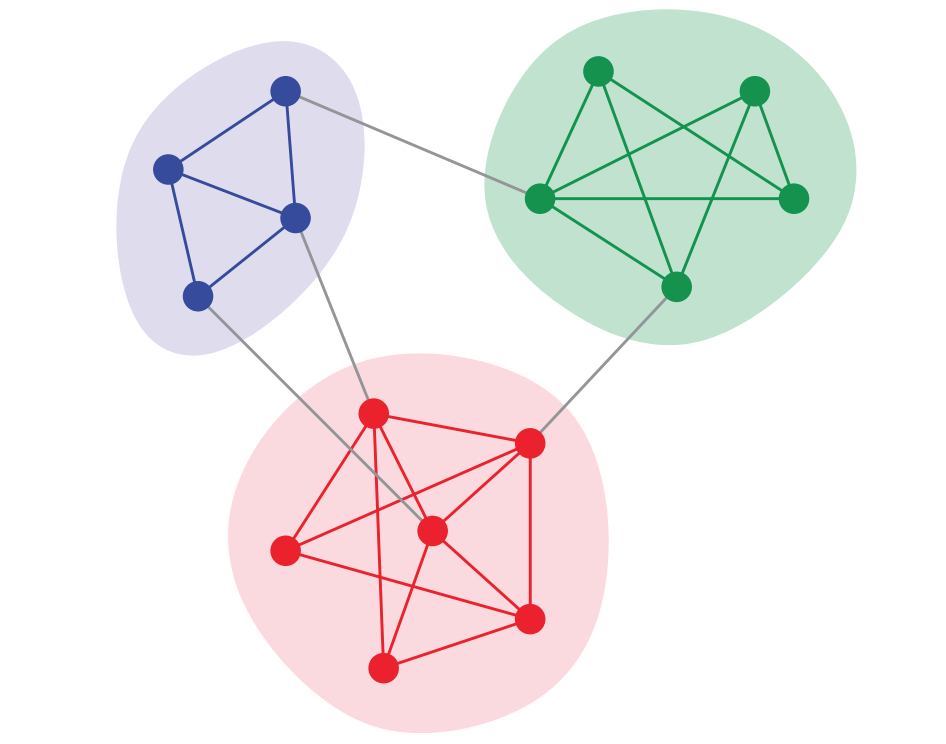
\includegraphics[width=0.5\columnwidth]{img/chapter1/community.png}
	%  \vspace{-1em}
	\caption{Example graph showing community structure. The nodes of this graph are divided into three communities, with most edges falling within communities and only a few between communities. The figure is contributed from \cite{newman2012communities}.}
	\label{fig:c1_community}
	%   \vspace{-1em}
\end{figure}
 

\begin{table}
	% \scriptsize
	\centering
	%   \vspace{-3em} 
	% \renewcommand{\tabcolsep}{2pt}
	\begin{tabular}{|p{3cm}|p{11cm}|} \hline
		\textbf{Term} &  \textbf{Definition} \\ \hline
		$G(V,E)$ & Graph $G$ with node set $V$ and edge set $E$.  \\ \hline
		$\Omega$ & $\Omega = \{ \omega_1,\omega_2,..., \omega_k\}$ is the ground truth community partition by models  where $\omega_k$ is the $k_{th}$ predicted community. \\ \hline
		$C$ & $C = \{ c_1,c_2,..., c_j\}$ is the detected community partition where $c_j$ is the $j_{th}$ community.\\ \hline
		$N, M$& $N = |V|$ denotes the node number and $M = |E|$ denotes the edge number in graph $G$\\ \hline
		$N_c$& $N_c = |c|$ is the number of nodes in community $c$\\ \hline
		$N_{c,\omega}$& $N_{c,\omega} = |c \cap \omega |$ is the common nodes in the detected community $c$ and ground truth community $\omega$ \\ \hline
		$E_{c}^{in}$& The number of edges within the community $c$. $E_{c}^{in} = \{(u,v) \in E : u \in c, v \in c \}$\\ \hline
		$E_{c}^{out}$& The number of edges on the boundary of the community $c$. $E_{c}^{out} = \{(u,v) \in E : u \in c, v \notin c$ \textit{or} $ u \notin c, v \in c \} $\\ \hline
		$D(v)$& Degree of node $v \in V$ \\ \hline
		$D_c$& The sum of node degrees in community $c$ \\ \hline
		$\mathcal{N}(v)$ & The neighbour node set of node $v$ \\ \hline
		$A$ & Graph adjacent matrix \\ \hline
	\end{tabular}
	\caption{Glossary of technical terms.}
	\label{tab:c2_glossary}
	
\end{table} 
\section{Background and Motivation}
Graph mining is one of the fundamental research areas in artificial intelligence; in the recent decade, community detection continues to be an essential topic within graph mining. Community detection approaches group nodes into communities, which can be regarded as a coarser view of a graph and reveal the latent knowledge of nodes. This detected knowledge can be used to support further tasks such as link prediction or node profile construction. For example, detecting researcher communities in a scholarly graph can imply future collaboration between them, or offer paper/research recommendations to targeted users. In biology, community structure can be used to infer possible protein-protein binding relationships, which may potentially contribute to healthcare. Therefore, exploring community detection tasks has huge practical value in both academic and industrial scenarios.

The popularity of community detection research is suggested by the thousands of papers published on the subject in top-tier journals and presented at conferences. Among these, some are survey papers which summarize state-of-the-art models from different perspectives; these have served as great references for me to organize relevant papers into different categories. \cite{fortunato2010community, fortunato2016community, coscia2011classification} are general survey papers which broadly introduce the definition of community detection and several types of models. Other papers pay more attention to detecting communities in particular types of graph. For example, \cite{malliaros2013clustering} is a classic paper which summarizes community detection in directed graphs; \cite{harenberg2014community} particularly focuses on large-scale graphs with empirical studies; and \cite{kim2015community} particularly summarizes the latest community detection models for multi-layer graphs. Still other papers focus on particular types of model frameworks. For example, \cite{abbe2017community} is the most recent work on block models in community detection. \cite{xie2013overlapping,amelio2014overlapping} are both authentic survey papers on overlapping community detection, even though they are slightly dated as of 2020.  \cite{nascimento2011spectral} is a classic research work that introduces a collection of spectral clustering models. To demonstrate how community detection supports interdisciplinary research efforts, \cite{javed2018community} and \cite{bedi2016community} show the application of community models to social media mining as well as other domains such as biology and neuroscience. Finally, \cite{chakraborty2017metrics} summarizes all types of evaluation metrics for model performance comparison. 

However, all of the aforementioned papers are either slightly out of date or relevant only to a specific topic; what is lacking is an effort to summarize and track the latest works from all possible main perspectives. This inspired me to include the most representative papers in this thesis, categorized by my own defined taxonomy. Specifically, derived from all existing works, I aim to leverage in-depth analysis in some subtle tasks and propose novel models to improve current model performance. A survey of the existing literature also inspired me to formulate and solve the various research questions mentioned in the following section.
\section{Research Problems}
In this section,I introduce three motivating tasks which this thesis aims to solve and briefly discuss my proposed approaches. The first task is \textit{Personalized Community Detection}, in which communities with different resolutions are formed given user information need. The second task is \textit{Cross-Graph Community Detection}, in which I detect pairwise user community closeness in sparse graphs by leveraging propagated information from external graphs. The third task is \textit{Community-Aware Dynamic Product Summarization}, in which community  is applied as supportive information to generate temporal product summarizations across different time periods. Details of my proposed models, along with extensive experiments and discussions, are introduced in the following chapters.

\subsection{Personalized Community Detection}
From a user-centric viewpoint, the ideal communities should provide a high-resolution partition in areas of the graph relevant to the user’s needs and a coarse partition on the remaining areas so as to best respond to the user’s needs (which can be formulated as a ``query'') in concentrated areas while leaving irrelevant areas less precisely specified. 

For instance, in Figure \ref{fig:example}, two different scholars in \textit{education} and \textit{data mining} domains, respectively, may consume the same scholarly graph differentlybecause they may need more detailed community exploration in their own domains whereas generalized community information is sufficient in irrelevant domains. For instance, a \textit{data mining} scholar may need more detailed communities in areas such as deep learning, graph mining, and Bayesian analysis, but for an \textit{education} researcher it may suffice to generalize these as computer science or even just science.

\begin{figure}
	% \setlength{\belowcaptionskip}{-10pt}
	\center
	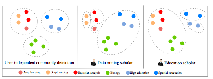
\includegraphics[width=0.8\columnwidth]{img/chapter3/example.pdf} 
	\caption{An example of personalized community detection on a scholarly graph} 
	\label{fig:example}
\end{figure}  

To solve this problem, I propose a \textbf{g}enetic \textbf{P}ersonalized \textbf{C}ommunity \textbf{D}etection (gPCD) model with an offline and an online step to efficiently cope with the time complexity issue in personalized community detection.  Details of the model structure are given in Chapter \ref{ch:personalized}.

\subsection{Cross-Graph Community Detection}
For a vulnerable graph with sparse connectivity, however, existing community detection algorithms can hardly probe enough information to optimize the community structure. Unfortunately, in real cyberspace this is a very common problem: while a handful of giant players (e.g., Google, Facebook, and Amazon) maintain high-quality graphs, thousands of apps are suffering from a “cold-start” problem in this area. If many users are isolated because of data sparseness, I can hardly determine any community information. 

To cope with this challenge, in this thesis I propose a novel research problem: Cross-Graph Community Detection. The idea is based on the fact that an increasing number of small apps are utilizing user identity information inherited from giant providers; for instance, users can easily log in to a large number of new apps using Facebook and Google ID. In such an ecosystem, the large main graph can provide critical information to enlighten community detection in many small sparse graphs. Figure \ref{fig:c4_example}depicts an example in which the Cooking and Cosmetic apps inherit important topological information from the main Amazon graph for enhanced community detection.

\begin{figure}  
	% \advance\leftskip-1cm 
	% \hspace*{0.25cm} 
	\centering
	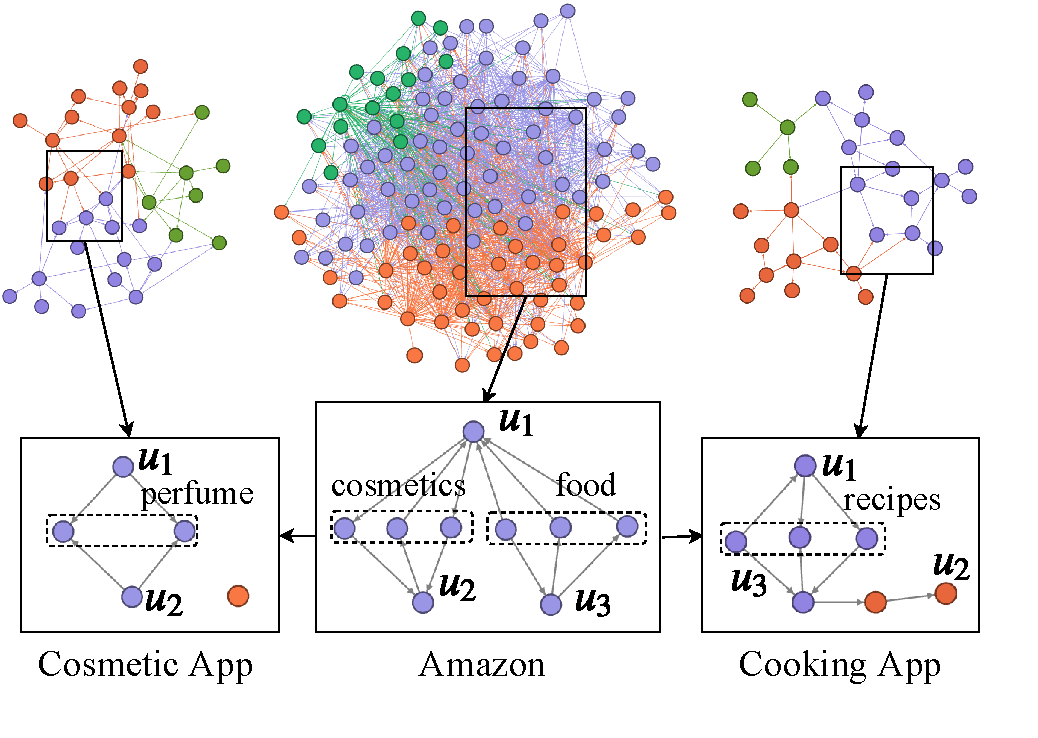
\includegraphics[width=0.8\columnwidth]{img/chapter4/example.pdf}
	%  \vspace{-1em}
	\caption{The Amazon graph is a main shopping graph while the Cosmetic App and the Cooking App are two small sparse graphs. Those graphs share mutual users in which three of them are selected to demonstrate their behaviors. Node colors indicate their related communities. }
	\label{fig:c4_example}
	%   \vspace{-1em}
\end{figure}

Inspired by the foregoing discussion, I propose an innovative \textit{Pairwise Cross-graph Community Detection} (PCCD) model for enhanced sparse graph user community detection. Specifically, given user $u_i$ and its associated triplet $\langle u_{i},u_{j},u_{k}\rangle$, I aim to predict the pairwise community relationships, e.g., compared with user $u_{k}$, does user $u_{j}$ have closer, similar or farther community closeness to user $u_i$? The details of this model structure are mentioned in Chapter \ref{ch:cross-graph}.

\subsection{Community-Aware Dynamic Product Summarization}
Product communities can implicitly reflect product characteristics. Therefore, understanding product communities and tracking their changes in a timely manner can support better decision-making for commercial purposes, such as informing online retailers in creating timely sales plans. Therefore, the \textit{Dynamic Community-Aware Product Summarization} task is of great importance. Such summarization not only indicates products’ dynamic membership changes but also utilizes these changes to depict product characteristics in readable contexts for easier interpretation.

\begin{figure}  
	% \advance\leftskip-1cm 
	\centering
	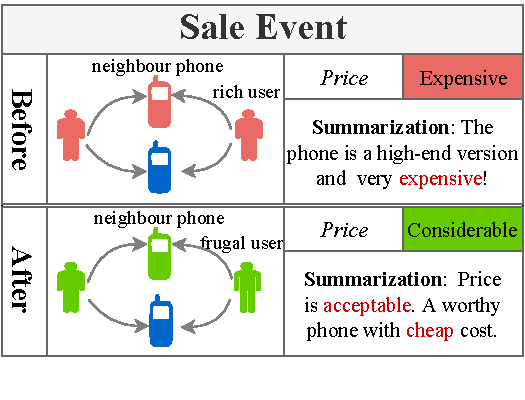
\includegraphics[width=0.8\columnwidth]{img/chapter5/example.pdf}
	% 	\vspace{-1em}
	\caption{An example to illustrate how to dynamically detect communities and select within-community neighbor products (red phone $\rightarrow$ green phone) for depicting current product (blue phone) characteristic change before \& after a sale event from user behaviors.}
	\label{fig:c5_example}
	% 	\vspace{-1.5em} 
\end{figure}

However, existing generative models relying on reviews inevitably face the sparsity issue: few products can gain enough reviews in a short time to depict the product’s temporal characteristics. User behaviors, on the other hand, are abundant and highly related to the product’s nature. Therefore, instead of review-based product summarization, I aim to generate community-aware product summarization in a dynamic manner. These approaches share the same goal but have huge differences in terms of proposed models. Review-based summarization directly runs a sequence-to-sequence model to generate product summarization by simply leveraging review context information. A community-aware product summarization, however, is generated from within-community neighbor product reviews. This means that it is a two-step approach, requiring both community detection and summarization generation.

As Figure \ref{fig:c5_example} depicts, when a sale event on a high-end phone brings frugal users' instant \textit{clicks}, behavior-based algorithms can immediately consume this information and locate updated within-community neighbor products (red phone $\rightarrow$ green phone) whose sufficient reviews help to update the product (blue phone) summarization. For review-based approaches, accumulating enough reviews to characterize this dynamic change may take a longer time. 

In the end,  I propose a  \textbf{B}ehavior based \textbf{D}ynamic \textbf{S}ummarization (BDS) model to accommodate user behavior for dynamic product summarization. The proposed model uses learned communities as a criteria to select neighbor products via a reinforcement approach, where textual review information is used to generate target product summarizations in a timely manner. Details of the model structure are given in Chapter \ref{ch:community-aware}.
\section{Contribution}
explain the contribution of this thesis such as categorizing the community detection into several forms, solve the three research questions, etc.
\section{Thesis Structure}
each chapter tells what.








